\documentclass[TFM.tex]{subfiles}

\begin{document}


\chapter{Proof of Deligne Conjecture}

Now that we know the quasi-isomorphism $C_*(E_2)\simeq H_*(E_2)$, we can prove the Deligne conjecture if we find an action of $H_*(E_2)$ on the Hochschild complex $C^*(A;A)$ inducing the Gerstenhaber algebra structure on $H^*(A;A)$. In this section, we will denote $G=H_*(E_2)$. For an operad $\OO$ of a certain kind that we will call \emph{quadratic}, there is an operad $\OO_\infty$ and a map $\OO_\infty\to\OO$, which is a quasi-isomorphism under certain conditions that $G$ satisfies, so we have a quasi-isomorphism $G_\infty\to G$. From this point, the idea is to factor this map through
\[
G_\infty\to \BB,\BB\to G
\]
where $\BB$ is an operad which acts on $C^*(A;A)$ inducing the Gerstenhaber algebra structure on $H^*(A;A)$.  This map won't be constructed explicitly since it relies on an isomoprhic operad $\widetilde{\BB}\cong\BB$, which is obtained using tools of Etingof-Kazhdan quantization theory \cite{EK} (see also Section 7 of \cite{Hinich}). Finally, since $\BB\simeq G$, we obtain the wanted action of $G$ on $C^*(A;A)$. 

Throughout this section $k$ is a field of characteristic 0. 


\section{Cooperads and coalgebras}

In order to define $G_\infty\to G$ we need some general constructions. All the following definitions can be found in \cite{Hinich}.

\begin{defi}
Let $M$ be a monoidal category ($M=\Vect, \Vectgr,\Ch$). An \emph{$\mathbb{S}$-object} in $M$ is a collection $X=\{X(n)\}_{n\geq 0}$ of objects of $M$ endowed with a right action of the symmetric groups $\Sigma_n$.
\end{defi}

Note than an operad $\OO$ is just an $\mathbb{S}$-object endowed with
equivariant operations
\[\OO(k)\otimes\OO(j_1)\otimes\cdots\otimes\OO(j_k)\to \OO(j_1+\cdots+j_k)\]
and with a unit element $1 \in\OO$ satisfying natural associativity and unit conditions.


\begin{defi}
Let $\OO$ be an operad in a symmetric monoidal category $M$. Let $V$ be an $\mathbb{S}$-object in $M$. The free $\OO$-algebra generated by $V$ is defined to be
\[
\F_\OO(V)=\oplus_{n\geq 0}\OO(n)\otimes_{\Sigma_n}V^{\otimes n}
\]
with a canonical $\OO$-algebra structure. EL GRUPO SIMÉTRICO AHÍ QUÉ SIGNIFICA Y CUÁL ES LA ESTRUCTURA CANÓNICA (NECESITARÍA APLICACIONES DE CADA PRODUCTO TENSORIAL A V)
\end{defi}

One has a forgetful functor from the category of operads to the category of $\mathbb{S}$-objects. This functor admits a \emph{free operad functor} as left adjoint \cite{GJHinich}. The free operad on an $\mathbb{S}$-object $X$ is denoted $\T(X)$ and can be thought as the operad generated by all formal operations corresponding to elements of each $X(n)$ and no relations between them.

Since the notions of operad and algebra can be defined in purely categorical terms, they can be dualized. Thus, a cooperad in $M$ is
the same as an operad in the opposite category $A^{op}$. Similarly one defines a coalgebra over a cooperad.

%LO DE NILPOTENTES CREO QUE NO LO NECESITO

\begin{defi}
If $V$ is an $\mathbb{S}$-object in $M$ and $\DD$ a cooperad in $M$. The \emph{cofree coalgebra cogenerated by }$V$ is defined to be
\[
\F^*_\DD(V)=\oplus_{n\geq 0}\left(\DD(n)\otimes V^{\otimes n}\right)^{\Sigma_n}
\]
EL SIGMA AHÍ QUÉ ES
\end{defi}

Let $X$ be a $\DD$-coalgebra and $V$ be an $\mathbb{S}$-object. Any map $X\to V$ of $\mathbb{S}$-objects defines canonically a map of $\DD$-coalgebras $X\to \F_\DD^*(V)$.  

The cofree cooperad cogenerated by $V$ is denoted $\T^*(V)$, and it is isomorphic to $\T(V)$ as an $\mathbb{S}$-object. 

\begin{remark}
Let $\OO$ be an operad of graded vector spaces such that the $\OO(n)$ are all finite dimensional. The, the collection of dual spaces $\{\OO(n)^*\}$ has an obvious cooperad structure. This cooperad is denoted $\OO^*$. Coalgebras over $\OO^*$ are sometimes called $\OO$-coalgebras. In the same style, we will sometimes write $\F^*_\OO(V)$ instead of $\F^*_{\OO^*}(V)$ since this object is a coalgebra over a cooperad, and therefore there is no confusion.
\end{remark}

\begin{defi}
An operad $\OO$ of graded vector spaces is called \emph{quadratic} if it is generated as an operad by $\OO(2)$ and relations spanned by composition of two binary operations (equivalently, the set of relations lies in $\OO(3)$). 
\end{defi}

In chapter 1 we explained that $G=H_*(E_2)$ was generated by $G(2)=H_*(E_2(2))$ and their relations involved compositions of $\mu$ and $l$ as we saw in the previous chapter. This shows that $G$ is quadratic. %en cada composición intervienen 2, no hay una tirple composición

\begin{defi}
Let $\OO$ be a quadratic operad with $V=\OO(2)$ and space of relations $R$. The \emph{dual cooperad} $\OO^{\perp}$ is cogenerated by the space $V[1]$ with corelations $\OO^\perp(3)=R[2]$ EL SHIFT DE ÍNDICES NO ENTIENDO POR QUÉ NI QUE SEA ASÍ
\end{defi}

\begin{defi}
Let $\OO$ be a (graded) quadratic operad. A structure of $\OO_\infty$-operad on $X\in\Vectgr$ is given by a differential on the cofree $\OO^\perp$-coalgebra cogenerated by $X$.
\end{defi}

The above definition gives rise to an operad $\OO_\infty$ in the category of complexes of graded vector spaces over $k$ as we're goint to see. In the case of $G_\infty$-algebras, there is an explicit definition than can be found in \cite[Proposition 16]{Galvez}. SI ME DA TIEMPO PONERLA EN ALGÚN LAO, AUNQUE REQUIERE VARIAS COSAS PREVIAS COMO TENGO POR AHÍ ABAJO EN MAYÚSCULAS COMENTADO

Let $X$ have a structre of $\OO_\infty$-algebra. The differential
\begin{equation}\label{9}
Q:\F^*_{\OO^\perp}(X)\to \F^*_{\OO^\perp}(X)[1]
\end{equation}
is defined uniquely by its composition with the projection onto the degree one component $\F^{*1}_{\OO^\perp}(X)=X$. ¿POR QUÉ? Thus, the differential is given by the collection of maps
\[
Q_i:\F^{*i}_{\OO^\perp}(X)=(\OO^\perp(i)\otimes X^{\otimes i})^{\Sigma_i}\to X[1].
\]
In particular, $d=Q_1$ defines a differential on $X\in\Vectgr$. COMO EL DUAL ESTÁ SHIFTEADO EL DE 1 ES COMO SI FUERA EL DE 0 QUE ES K Y POR ESO SALE.

Define $\OO_\infty=\T(\OO^\perp)$ to be the free graded operad generated by $\OO^\perp$ (as $\mathbb{S}$-object). The collection of
maps $Q_i$ defines an action of $\OO_\infty$ on $X$. We have the following lemma ME GUSTARÍA UNA REFERENCIA PORQUE HINICH NI LO PRUEBA NI LO REFERENCIA, ADEMÁS LUEGO EN EL EJEMPLO DEFINE UNA DIFERENCIAL, PERO NO SABEMOS SI PARA ESA VALE QUE $Q^2=0$ IMPLIQUE QUE $Q$ RESPETA LAS DIFERENCIALES

%LO DE LA DIFERENCIAL ME HACE FALTA PARA QUE LA APLICACIÓN RESPETE LAS DIFERENCIALES Y SEA DE VERDAD UN MORFISMO DE ALGEBRAS EN COMPLEJOS DE CADENAS
Nextt, we have the following lemma.
\begin{lemma}
There exists a unique differential on the graded operad $\OO_\infty$ such that the condition $Q^2=0$ for a degree one differential $Q$ as in \ref{9} is equivalent to the statement that the action of $\OO_\infty$ on $(X,d=Q_1)$ respects the differentials. 
\end{lemma}


\begin{ex}
Let $X$ be a complex endowed with a $\OO$-algebra structure (dg $\OO$-algebra). Define the differential $Q$ on $\F^*_{\OO^\perp}(X)$ as follows.

$Q_1:X\to X[1]$ is the differential of $X$. $Q_2:\OO^{\perp}(2)\otimes X^{\otimes 2}\to X[1]$ is defined by the $\OO$-algebra structure on $X$ since $\OO^\perp(2)=\OO(2)[1]$. For $i>2$, $Q_i$ are defined to be 0. 

The condition $Q^2=0$ can be easily verified since we're assuming that $\OO$ is quadratic. This means that any $\OO$-algebra admits a canonical $\OO_\infty$-algebra structure. 
\end{ex}

The last example shows that there is a canonical map of operads in $\Ch$
\begin{equation}\label{map}
\OO_\infty\to \OO.
\end{equation}
DICE HINICH QUE SUPONE QUE O TIENE DIFERENCIAL 0 PERO NO VEO LA NECESIDAD.

\begin{defi}
A quadratic operad $\OO$ is called \emph{Koszul} if the map \ref{map} is a quasi-isomorphism.
\end{defi}

Hinich \cite{Hinich} shows that $G$ is Koszul using Kähler differentials and other techniques that we won't describe here. That fact is also proved in \cite{GJHinich}. Another approach using that $G_\infty$ is the \emph{Koszul resolution} of $G$ is presented in \cite{AlgebraicOperads}. In any case, we have a quasi-isomorphism
\begin{equation}
G_\infty\xrightarrow{\simeq} G.
\end{equation}

%AQUÍ LO QUE PUEDA SACAR DE HINICH

%\url{https://en.wikipedia.org/wiki/Bialgebra}
%
%\url{https://en.wikipedia.org/wiki/Coalgebra}

%SECCIÓN 5.5 (CREO QUE PUEDO ESQUIVAR LO DE DG BIALGEBRA DANDO DIRECTAMENTE LA ESTRUCTURA EN EL GRADED VECTOR SPACE)

%CREO QUE DE 6 ME LO PUEDO SALTAR, PORQUE AUNQUE CONSTRUYE LA APLICACIÓN, REQUIERE LAS CONSTRUCCIONES RARAS DEL PRINCIPIO (SALVO QUE EN ALGÚN MOMENTO LAS ENTIENDA, TIENEN UNA DESCRIPCIÓN EXPLÍCITA EN LAS PÁGINAS 5-6 PERO NO SÉ QUÉ REPRESENTA $S_n$ EN CADA CASO) ASÍ QUE SOLO COMENTAR QUE HACE FALTA LO DE ETINGOF-KAZHDAN


%EN ALGUNO DE LOS PAPERS PONE QUE KOSZUL ES CUANDO ES CUADRÁTICA (GENERADA POR LA OPERACIÓN DE GRADO 2) Y LAS RELACIONES ESTÁN EN $V\oplus (V\otimes V)$ ASÍ QUE ENTIENDO QUE VALENCIA 0 ES EN EL CUERPO Y POR ESO VALENCIA 3 ES AHÍ

%QUIÉN COÑO ES $G_\infty$? ¿ES SIMPLEMENTE PONERLE EL INFINITO COMO EN 3.1.4 (PARA LO CUAL TENGO QUE ENTENDER MEJOR LAS CONSTRUCCIONES ESAS DE MIERDA)? (Y DE ALGÚN MODO SALE EL OPERAD, QUIZÁ POR LO QUE SE CUENTA ANTES COMO LAS CONMUTATIVAS Y LAS ASOCIATIVAS Y LAS LIE) EN ESE CASO EL EJEMPLO 3.1.7 DARÍA YA UNA APLICACIÓN $G_\infty\to G$ PERO SUPONGO QUE HAY QUE DE TODOS MODOS HAY QUE PROBAR QUE SE TIENE UNA APLICACIÓN QUE ES EQUIVALENCIA

---------------------------------------------------------------------------------------------------------------------

%PARA DESCRIBIR $G_\infty$ (AUNQUE COMENTARÉ QUE SE PUEDE DESCRIBIR COMO LA RESOLUCIÓN DE KOSZUL DE $G$): GALVEZ-CARRILLO PROPOSITION 16 PAGINA 559 (21 DEL PDF). PRIMERO NECESITO LA DEFINICIÓN DE S DE LA CONVENCIÓN 0.1 EN LA PÁGINA 542 (4 DEL PDF), PARA LA BARRA PÁGINA 554 (16 DEL PDF). AUNQUE TENIENDO EN CUENTA QUE NO ME DA LA APLICACIÓN A $G$, CREO QUE ME TRAE MÁS CUENTA TRATAR DE HACERLO COMO HINICH, QUE NO ES TAN COMPLICADO DE DEFINIR, SOLO DE ENTENDER, PERO CREO QUE PUEDO (Y COMENTAR QUE EN GALVEZ-CARRILLO ESTÁ MÁS EXPLÍCITO)

%LA PROPIEDAD DE QUE SEA UN QUASISOMORFISMO ES PARA QUADRATIC OPERAD (ALGEBRAIC OPERADS 7.1.1)

\section{Operad $\BB$ and its action on the Hochschild complex}
We shall now describe an operad which
acts naturally on the Hochschild complex of any associative algebra. This operad is
usually denoted $\BB_\infty$ (see \cite{Hinich}), but since it is not obtained by Koszul resolution of any operad $\BB$, we will denote it $\BB$. 

In this section $A$ is any associative $k$-algebra and $\CC=C^*(A;A)$.
It is convenient to denote elements $f \in \CC^n$ as boxes having $n$ inputs and one output like
this:

\begin{figure}[h!]
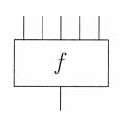
\includegraphics[scale=0.9]{Imagenes//box}
\end{figure}


\begin{defi}
Let $f,g_1,\dots, g_n\in \CC$. Denote the \emph{brace} $f\{g_1,\dots, g_n\}$ by the following formula.

\begin{figure}[h!]
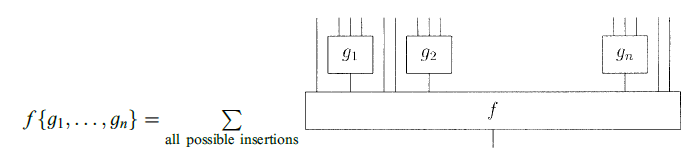
\includegraphics[scale=0.7]{Imagenes//brace}
\end{figure}

Here the sum is taken over all possible order preserving insertions of outpus of $g_i$ into
inputs of $f$.
\end{defi}

\begin{remark}
We have chosen to use pictures in the previous definition in order to avoid unpleasant
signs in formulas. The signs reappear if one decides to write down the expression for
$f\{g_1,\dots, g_n\}(a_1\otimes \cdots \otimes a_m)$, compare to \cite{GJHinich}, Formula (1) on p. 49.
\end{remark}

The Lie bracket on $\CC$ is given explicitly, in terms of braces, by the formula %pone \CC[1] porque es de grado 1
\[
[f,g]=f\{g\}-(-1)^{|f||g|}g\{f\}.
\]
%en la sección 6 de Gerstenhaber sale la composición con la cual [f,g] es el conmutador, que consiste precisamente hacer las inserciones


\begin{defi}
A $\BB$-algebra structure on a graded vector space $X$ is given by the following operations: PREGUNTAR POR LAS TRANSFORMACIONES QUE HACE PARA LLEGAR A LA DEFINICIÓN QUE ESTOY PONIENDO PORQUE IGUAL NO TIENE SENTIDO DECIR QUE LAS QUE SALEN SON DIFERENTIAL DE GRADO 1
\begin{itemize}
\item differentials of degree 1 $m_n:X^{\otimes n}\to X[2-n]$.
\item multiplications of degree 0 $m_{pq}:X^{\otimes p}\otimes X^{\otimes q}\to X[1-p-q]$.
\end{itemize}
Therefore, the $\BB$-structure is given by a collection of operations $m_n$ and $m_{pq}$
subject to some relations. This defines an operad $\BB$ as the one generated by $m_n\in\BB(n)^{2-n}$ and $m_{pq}\in\BB(p+q)^{1-p-q}$ subject to some relations. LOS SUPERÍNDICES
\end{defi}

\subsection{Action of $\BB$ on $C^*(A;A)$}
We have to define the action of the operations
$m_n$ and $m_{pq}$ on $C^*(A;A)$ and to check the compatibilities. The action is given below.
\begin{itemize}
\item $m_1$ is the differential in $\CC$. 
\item $m_2$ is the multiplication $m:\CC\otimes\CC\to\CC$ defined by the formula $m(x\otimes y)=\mu(x\boxtimes y)$, where $\mu$ is the multiplication $\mu:A\otimes A\to A$ and $x\boxtimes y:A^{\otimes m+n}\to A^{\otimes 2}$ is the tensor product of maps $x:A^{\otimes m}\to A$ and $y:A^{\otimes n}\to A$.
\item $m_i=0$ for all $i>2$.
\item $m_{1k}(f\otimes g_1\otimes\cdots\otimes g_k)=f\{g_1,\dots, g_k\}$.
\item $m_{kl}=0$ for $k>1$.
\end{itemize}
Note that this action is equivalent to an action of an operad $\BB_0$ defined like $\BB$ but declaring $m_i=0$ for $i>2$ and $m_{kl}=0$ for $k>l$ in the first place. This operad $\BB_0$ can be seen as a \emph{quotient} of $\BB$ by the stated relations. 

POR LO DE ARRIBA $M_2$ CREO QUE DEBERÍA SER UNA DIFERENCIAL TAMBIÉN (PEDIR DE TODAS FORMAS LA REFERENCIA QUE DECÍA MURO PARA LA ACCIÓN Y A VER SI AHÍ SE VE QUE SE INDUCE LA DE GERSTENHABER, AUNQUE ME DA LA SENSACIÓN DE QUE ES EVIDENTE, PORQUE TIENES LA DIFERENCIAL, LA MULTIPLICACIÓN Y EL CORCHETE QUE SALE CON EL BRACE, AUNQUE PARECERÍA QUE SALDRÍAN MÁS COSAS CON EL CORCHETE CUANDO HAY MÁS DE UNA G)

SE SUPONE QUE HABRÍA QUE COMPROBAR QUE ESO PRODUCE ESTRUCTURA DE B-ALGEBRA PERO TENGO QUE ENTENDER BIEN LO DE ARRIBA


\end{document}